% Braking envelope: piecewise-linear inner approximation of sqrt(v_f^2 + 2 a_b d)
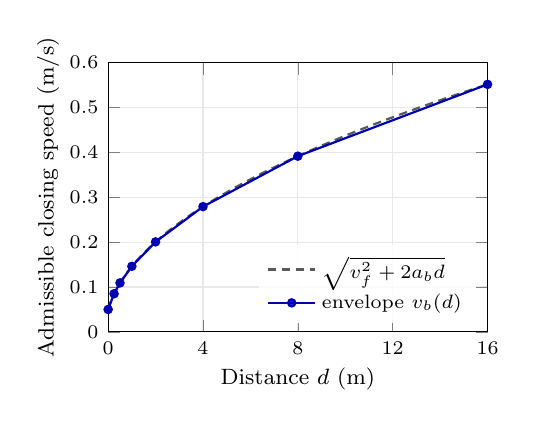
\begin{tikzpicture}[font=\footnotesize]
\begin{axis}[
  width=6.4cm, height=5.0cm,
  xmin=0, xmax=16, ymin=0, ymax=0.6,
  xtick={0,4,8,12,16}, ytick={0,0.1,...,0.6},
  yticklabel style={/pgf/number format/fixed,/pgf/number format/precision=1},
  xlabel={Distance $d$ (m)}, ylabel={Admissible closing speed (m/s)},
  xlabel style={yshift=2pt}, ylabel style={yshift=-3pt},
  tick label style={font=\scriptsize},
  legend style={font=\scriptsize,at={(0.97,0.03)},anchor=south east,draw=none,fill=white,fill opacity=0.85,text opacity=1},
  legend cell align=left,
  grid=major, grid style={gray!18}]
\addplot[densely dashed,gray!70!black,thick,domain=0:16,samples=200] {sqrt(0.05^2 + 2*(0.5*2/106)*x)};
\addlegendentry{$\sqrt{v_{f}^{2}+2a_{b}d}$}
\addplot[blue!70!black,thick,mark=*,mark size=1.3pt] coordinates {
  (0,0.0500) (0.25,0.0850) (0.5,0.1092) (1,0.1462) (2,0.2006) (4,0.2792) (8,0.3917) (16,0.5517)};
\addlegendentry{envelope $v_{b}(d)$}
\end{axis}
\end{tikzpicture}
